\section{Implementação}

Toda a parte de processamento de imagem se encontra no código fonte \texttt{lib.py}. Cada subseção mostra no trecho de código qual função nesse arquivo se encontra a implementação da operação. Os trechos apresentados refletem o código no arquivo, mas sem detalhes como cópias de \textit{buffer} e tipagem estática.

Quando possível, a função equivalente do OpenCV também será apresentada, já que as acelerações de GPU podem ser mais facilmente acessadas usando \pyline{cv2.cuda} em vez de apenas \pyline{cv2} \autocite{ref:cvcuda}. Entretanto, as operações foram implementadas apenas com Numpy neste trabalho, visando a familiarização com técnicas de vetorização.

Assuma que as bibliotecas são importadas como:

\begin{minted}{python}
    import numpy as np
    import cv2
\end{minted}

\subsection{Conversão para Monocromático}

A transformação para escala de cinza é feita através da média dos três canais de cores, truncada para inteiro. A matriz resultante é então repetida novamente para os três canais, para que a operação possa ser repetida sem erros de execução do programa.

\begin{listing}[h]
    \caption{Comando \texttt{monocromatico}}

    \begin{minted}{python}
        def grayscale(imagem):
            gray = np.mean(imagem, axis=2).astype(np.uint8)
            return np.stack([gray, gray, gray], axis=2)
    \end{minted}
\end{listing}

\begin{figure}
    \centering
    \begin{subfigure}{0.45\textwidth}
        \centering
        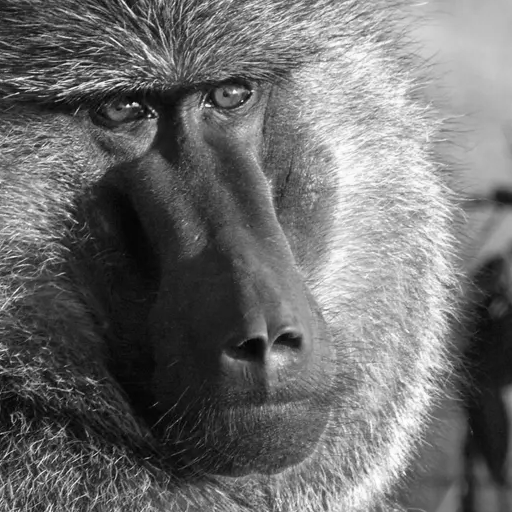
\includegraphics[width=6cm]{resultados/colormono.png}
        \caption{\texttt{imagens/color.png}}
    \end{subfigure}%
    \begin{subfigure}{0.45\textwidth}
        \centering
        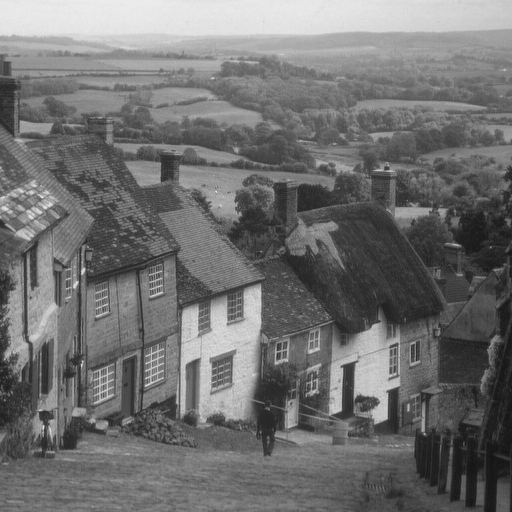
\includegraphics[width=6cm]{resultados/citymono.png}
        \caption{\texttt{imagens/city.png}}
    \end{subfigure}

    \caption{Mudaça para escala de cinza.}
\end{figure}

Em vez de \pyline{np.mean(imagem, ...)}, a conversão poderia ser implementado também com \pyline{cv2.cvtColor(image, cv2.COLOR_BGR2GRAY)} \autocite{ref:cvtcolor}.

\subsection{Negativo da Imagem}

Para essa conversão basta fazer ~\pyline{255 - intensidade}~ para cada píxel. Como 255 também é o maior valor de um \textit{byte}, basta também inverter todos os bits da imagem.

\begin{figure}[H]
    \centering
    \begin{subfigure}{0.45\textwidth}
        \centering
        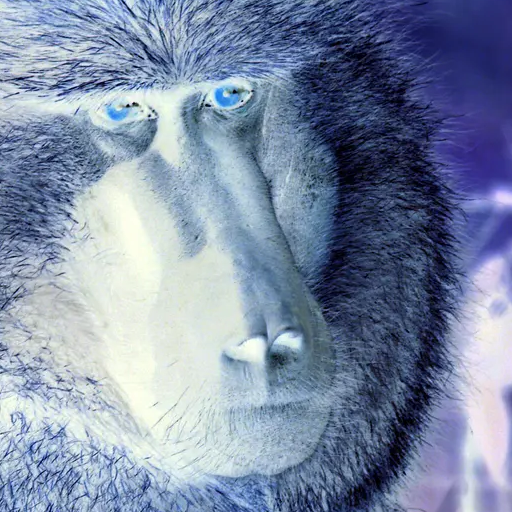
\includegraphics[width=6cm]{resultados/colorneg.png}
        \caption{\texttt{imagens/color.png}}
    \end{subfigure}%
    \begin{subfigure}{0.45\textwidth}
        \centering
        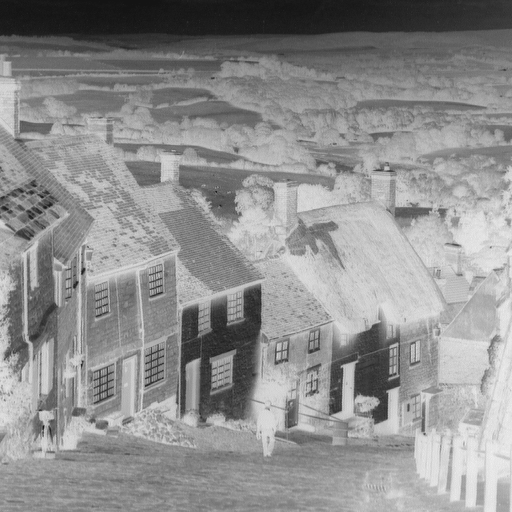
\includegraphics[width=6cm]{resultados/cityneg.png}
        \caption{\texttt{imagens/city.png}}
    \end{subfigure}

    \caption{Imagem com intensidade invertida.}
\end{figure}

\begin{listing}[H]
    \caption{Comando \texttt{negativo}}

    \begin{minted}{python}
        def negativo(imagem):
            return ~imagem
    \end{minted}
\end{listing}

Em vez de usar o \textit{not} do Numpy, existe também a função \pyline{cv2.bitwise_not(imagem)} \autocite{ref:bitwise_not}.

\subsection{Espelhamento Vertical}

\begin{listing}[h]
    \caption{Comando \texttt{esp.vertical}}

    \begin{minted}{python}
        def espelhamento_vertical(imagem):
            return imagem[::-1]
    \end{minted}
\end{listing}

\begin{figure}[h]
    \centering
    \begin{subfigure}{0.45\textwidth}
        \centering
        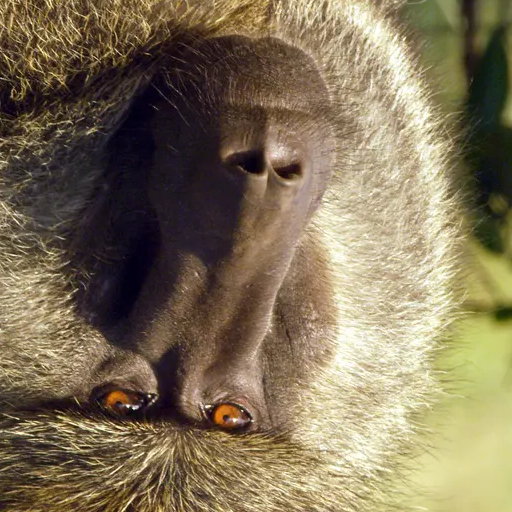
\includegraphics[width=6cm]{resultados/colorflip.png}
        \caption{\texttt{imagens/color.png}}
    \end{subfigure}%
    \begin{subfigure}{0.45\textwidth}
        \centering
        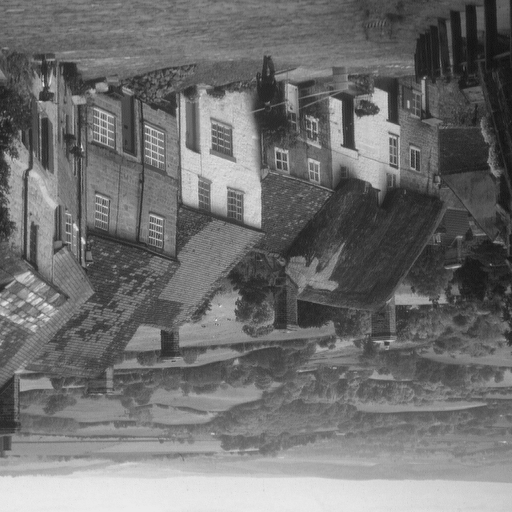
\includegraphics[width=6cm]{resultados/cityflip.png}
        \caption{\texttt{imagens/city.png}}
    \end{subfigure}

    \caption{Espelhamento vertical.}
\end{figure}

Pode ser implementado também com \pyline{cv2.flip(imagem, 0)} \autocite{ref:flip}.

\subsection{Mosaico} \label{sec:mosaico}

\textcolor{red}{ORDENACAO? PADRAO? IMPL?}

\begin{minted}{text}
    $ python main.py imagens/baboon.png mosaico padrao.txt
\end{minted}

\begin{figure}[H]
    \centering
    \begin{subfigure}{0.45\textwidth}
        \centering
        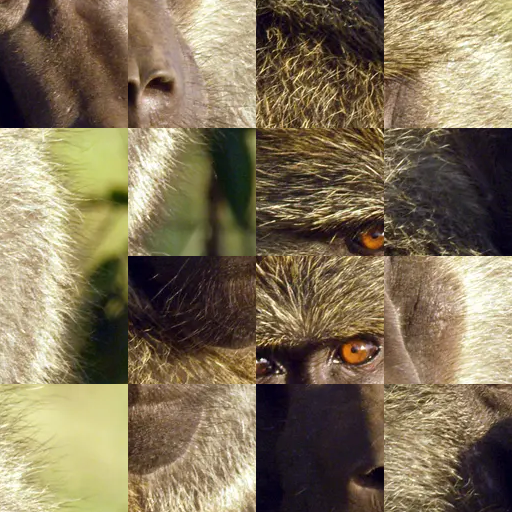
\includegraphics[width=6cm]{resultados/colormsc.png}
        \caption{\texttt{imagens/color.png}}
    \end{subfigure}%
    \begin{subfigure}{0.45\textwidth}
        \centering
        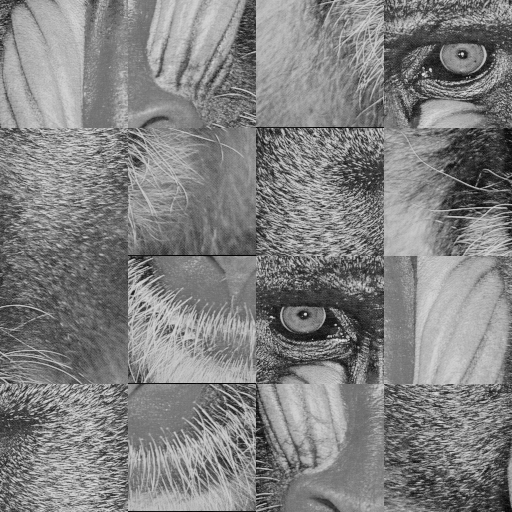
\includegraphics[width=6cm]{resultados/baboonmsc.png}
        \caption{\texttt{imagens/babooon.png}}
        \label{fig:res:10}
    \end{subfigure}

    \caption{Mosaico da imagem com \textcolor{red}{ALGUMA COISA}.}
\end{figure}

\begin{listing}[H]
    \begin{minted}{python}
        def mosaico(imagem, ordem):
            N, M = ordem.shape
            # split e flatten
            bloco = [
                bloco
                for lin in np.vsplit(imagem, N)
                for bloco in np.hsplit(lin, M)
            ]
            # accesso (em lista) e concatena
            imagem = np.concatenate([
                np.concatenate([bloco[i] for i in lin], axis=1)
                for lin in ordem
            ])
            return imagem
    \end{minted}

    \caption{Comando \texttt{mosaico ORDENACAO}}
\end{listing}

